\documentclass[border=5pt]{standalone}
\usepackage{tikz}
\usepackage{tikz-3dplot}
\usetikzlibrary{arrows.meta, 3d, perspective, calc, matrix, positioning}
\usepackage{amsmath}
\begin{document}
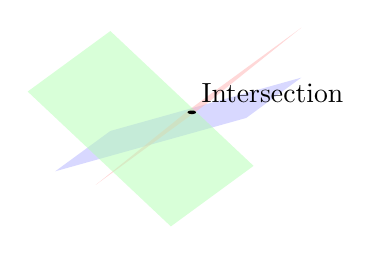
\begin{tikzpicture}[scale=0.7, >=stealth, 3d view={30}{25}]
    % Draw first plane
    \fill[blue!30,opacity=0.5] (-1,1,-1) -- (3,1,1) -- (3,3,1) -- (-1,3,-1) -- cycle;
    % Draw second plane
    \fill[red!30,opacity=0.5] (1,-1,0) -- (3,-1,2) -- (3,3,2) -- (1,3,0) -- cycle;
    % Draw third plane
    \fill[green!30,opacity=0.5] (-1,0,1) -- (2,0,-1) -- (2,3,-1) -- (-1,3,1) -- cycle;

    % Draw intersection point
    \fill[black] (1.67,1.33,0.67) circle (0.08) node[above right] {Intersection};

\end{tikzpicture}
\end{document}
